\documentclass[bwprint]{gmcmthesis}
\usepackage{amsmath}
\usepackage{pdfpages}
\usepackage{svg}
\numberwithin{figure}{section}
\renewcommand{\thefigure}{\arabic{section}-\arabic{figure}} 
\title{风电场有功功率优化分配}
\baominghao{No.2410*******} %参赛队号
\schoolname{XX大学}%学校名称
\membera{队员A} %队员A
\memberb{队员B} %队员B
\memberc{队员C} %队员C
\linespread{1.2}
\begin{document}
 \maketitle
\begin{abstract}
	针对风电场有功功率优化调度中的关键问题，本文围绕疲劳损伤实时量化、载荷间接估计、多目标优化调度及鲁棒性增强四个层次展开研究。
	\par 针对问题一，首先，基于 Palmgren-Miner 疲劳损伤理论建立风机主轴和塔架的累积疲劳损伤程度量化指标计算的数学模型。接着，基于三点式雨流计数法原理，利用滑动窗口内的载荷损伤对历史疲劳损伤进行累加，在CPU上实现每秒损伤值计算，计算时间<1s，且计算结果相似度良好。
	\par 针对问题二，基于风机的气动系统模型，建立了与风速和功率参考值相关的主轴扭矩和塔架推力计算模型，分别采用最小二乘法以及Levenberg-Marquardt算法拟合参数，拟合优度分别为0.9691和0.9999。
	\par 针对问题三，构建以主轴和塔架损伤均值最小化为双目标、满足功率平衡与偏差约束的优化模型，采用NSGA-II 算法每秒求解一次，取Pareto前沿中选择双目标之和最小的解，制作了动图每秒实时对比优化前后疲劳损伤。
	\par 针对问题四，基于卡尔曼滤波去噪，同时采用差分自回归移动平均（ARIMA）和 LSTM模型根据已有数据预测延迟信号并补偿时滞，提升优化模型的鲁棒性。

\keywords{滑动窗口；雨流计数法；NSGA-II 算法；卡尔曼滤波}
\end{abstract}
%\pagestyle{plain}
\tableofcontents
\newpage
\section{问题重述}
随着我国风电产业向大型化、规模化发展，额定容量更高的风机因机械部件柔性增强，导致疲劳损伤累积加快，不仅增加运维成本、降低发电效率，还可能引发倒塌、断裂等严重安全事故。因此，亟需通过优化控制手段降低风机运行中的累积疲劳损伤，从而延长设备寿命、减少非计划停机损失，并节约运维资源。
\par 在风电场实际运行中，电网调度指令 $P_t$每秒下发至场站自动发电控制系统（AGC），由AGC按一定分配策略将总功率分摊至每台风机（即功率参考值$P_{ref}^{i}$），各风机再精确跟踪该指令发电。传统上采用平均分配方法，即每台风机承担 $P_{ref}^{i}=P_t/W_t$，$W_t$为风机总数），但该方法未考虑各风机风速差异及疲劳状态，导致部分风机长期处于高疲劳负荷工况，影响整场运行安全与经济效益。故亟需建立更优的功率分配策略，在满足调度指令的同时，平衡和降低全场风机的累积疲劳损伤。本文聚焦于以下四个风电场有功功率优化调度问题：
\begin{enumerate}
	\item \textbf{疲劳损伤计算}：建立数学模型评估疲劳损伤；利用100台风机100秒的载荷（塔架推力与主轴扭矩）数据，输出每台风机的两种元件每秒实时疲劳损伤，计算时间<1s，且结果与雨流计数法趋势一致。
	
	\item \textbf{载荷计算}：根据风速和功率参考值，建立模型估算主轴扭矩和塔架推力，并与附件2提供的参考值对比，统计误差平方和。
	
	\item \textbf{调度优化}：目标为降低全场主轴和塔架总体疲劳损伤，建立优化模型（约束：功率平衡、额定功率限制、与平均分配偏差），实时求解并对比优化效果。
	
	\item \textbf{鲁棒优化}：考虑测量噪声（±10\%）和通信延迟（≤10s），改进问题三模型，在附加测试集上验证抑制能力。
\end{enumerate}

\section{模型假设}
\begin{itemize}
	\item 各风机型号相同，仅风速和功率参考值不同。
	\item 疲劳损伤满足Palmgren-Miner线性累积准则。
	\item 风能过剩（风速≥额定风速11.2m/s），风机始终可发额定功率。
	\item 风机机械功率转化为输出功率的效率为常数。
	\item 功率跟踪精确实现，忽略动态响应误差。
	\item 载荷数据采样周期为1s，损伤累积与循环周期解耦。
	\item 噪声服从零均值均匀分布，延迟为随机整数秒。
\end{itemize}
\newpage
\section{符号说明}
\begin{table}[h]
	\centering
	\caption{主要符号}
	\label{tab:symbols}
	\begin{tabular}{cc}
		\toprule
		\textbf{符号} & \textbf{含义} \\
		\midrule
		$P_t$ & 电网调度总功率指令（MW） \\
		$P_{ref}^i$ & 第$i$台风机的有功参考值（MW） \\
		$W_t$ & 场内风机总数（100台） \\
		$T_s^i$ & 第$i$台风机主轴扭矩（kN$\cdot$m） \\
		$F_t^i$ & 第$i$台风机塔架推力（kN） \\
		$D_s^i(t)$ & 第$i$台风机主轴$t$时刻累积疲劳损伤 \\
		$D_t^i(t)$ & 第$i$台风机塔架$t$时刻累积疲劳损伤 \\
		$\tilde{D}_s^i(t)$ & 第$i$台风机主轴$t$时刻累积疲劳损伤实时计算指标 \\
		$\tilde{D}_t^i(t)$ & 第$i$台风机塔架$t$时刻累积疲劳损伤实时计算指标 \\
		$N_s^i$ & 第$i$台风机的主轴扭矩最大循环次数 \\
		$N_t^i$ & 第$i$台风机的塔架推力最大循环次数 \\
		$n_s^i$ & 第$i$台风机的主轴扭矩应力循环次数 \\
		$n_t^i$ & 第$i$台风机的塔架推力应力循环次数 \\
		$v_i$ & 第$i$台风机风速（m/s） \\
		$\omega_r^i$& 第$i$台风机低速轴转速\\
		$\lambda_i$ &  第$i$台风机叶尖速比 \\
		$\beta_{i}$& 第$i$台风机叶桨距角\\
		$R$ & 风轮半径（m） \\
		$\rho$ & 空气密度（kg/m$^3$） \\
		$\eta$ & 转换效率\\
		$\alpha$ & 主轴损伤目标权重系数 \\
		$\gamma$ & 鲁棒优化中不确定性惩罚系数 \\
		\bottomrule
	\end{tabular}
\end{table}
\newpage
\section{模型建立与求解}
\subsection{问题一：疲劳损伤计算模型}
\textbf{疲劳损伤}\quad 设$\Omega^s_i(\tau), \Omega^t_i(\tau)$分别为第$i$台风机主轴扭矩和塔架推力在$\tau$时刻之前（含$\tau$时刻）所有循环的指标集。
根据Palmgren-Miner 线性累积损伤理论，第$i$台风机主轴和塔架在$\tau$时刻累积疲劳损伤分别为
\begin{equation}
	D_s^i(\tau)=\sum_{j\in\Omega^s_i(\tau)}\frac{n_s^i(j)}{N_s^i(j)},\quad D_t^i(\tau)=\sum_{j\in\Omega^t_i(\tau)}\frac{n_t^i(j)}{N_t^i(j)},
\end{equation}
其中单次循环时$n_s^i=n_t^i=1$，半次循环时$n_s^i=n_t^i=0.5$；$N_s^i(j)$和$N_t^i(j)$分别为第$i$台风机按照循环$j$的主轴扭矩和塔架推力相应的最大循环次数，满足
\begin{equation}
	(\hat{S}_s^i)^mN^i_s=(\hat{S}_t^i)^mN^i_t=C,
\end{equation}
其中Wohler指数$m=10$，$C=9.77×10^7$，$\hat{S}_s^i, \hat{S}_t^i$分别为修正（等效均值为0时）的主轴扭矩和塔架推力幅值，计算公式分别为
\begin{equation}
	\frac{S^{i}_{s}}{\hat{S}^i_s}+\frac{\bar{S}^i_{s}}{\sigma _b}=1, \quad \frac{S^{i}_{t}}{\hat{S}^i_t}+\frac{\bar{S}^i_{t}}{\sigma _b}=1,
\end{equation}
其中$\sigma_b$为材料在拉伸断裂时的最大载荷值，在本题中两种元件均为为50000000。${S}_s^i, {S}_t^i$分别为主轴扭矩和塔架推力幅值，$\bar{S}_s^i, \bar{S}_t^i$分别为主轴扭矩和塔架推力均值。
\par 采用\textbf{滑动时间窗口}实时计算疲劳损伤指标$\tilde{D}^i_t(\tau)$和$\tilde{D}^i_s(\tau)$，具体步骤如下：
\begin{enumerate}
	\item 初始时，$\tilde{D}^i_s(1)=\tilde{D}^i_t(1)=0$，$\tau=2$时为半循环，$\tilde{D}^i_s(2)={D}^i_s(2)$，$\tilde{D}^i_t(2)={D}^i_t(2)$。
	\item $3\leq \tau\leq10$时$\tilde{D}^i_s(\tau)=\max\{{D}^i_s(\tau), {D}^i_s(\tau-1)\}$，$\tilde{D}^i_t(\tau)=\max\{{D}^i_t(\tau), {D}^i_t(\tau-1)\}$。
	\item 当$\tau>10$时，计算循环时仅取当前时刻前$L=10$秒的载荷序列，然后叠加计算疲劳损伤，即$\tilde{D}^i_s(\tau)=\tilde{D}^i_s(\tau-1)+{D}^i_s(\tau)$，$\tilde{D}^i_t(\tau)=\tilde{D}^i_t(\tau-1)+{D}^i_t(\tau)$。
\end{enumerate}
\par 采用\textbf{三点式雨流计数法}统计循环。以第$i$个风机的主轴为例，具体步骤如下：
\begin{enumerate}
	\item 设定三个连续的应力状态点$S_1, S_2, S_3$作为分析单元。
	\item 计算这两段相邻的应力变化量$\Delta S_1 = \left|S_1 - S_2\right|$ 和 $\Delta S_2 = \left|S_2 - S_3\right|$。
	\item 当$\Delta S_1 \leq \Delta S_2$时，此时将$S_1$至$S_2$视为一个有效循环计数，然后跳至步骤5。计数方法：取$n_s^i=1$, 主轴扭矩幅值$S^i_s=\Delta S_1$，主轴扭矩均值 $\bar{S}^i_s=\frac{S_1+S_2}{2}$。
	\item 反之，若$\Delta S_1>\Delta S_2$，则当前三点组内不识别出循环，不予计数。继续取连续应力状态点$S_2, S_3, S_4$作为分析单元（若无$S_4$，则从序首$S_1$重新开始取，下同），跳至步骤2。若整个序列中仅剩少于3个应力状态点，跳至步骤6。
	\item 移除$S_1, S_2$，继续取连续的应力状态点$S_3, S_4, S_5$作为分析单元，跳至步骤2。若整个序列中仅剩少于3个应力状态点，跳至步骤6。
	\item 若序列中仅剩2个连续的应力状态点，取$n_s^i=0.5$, 主轴扭矩幅值$S^i_s=\Delta S_1$，主轴扭矩均值 $\bar{S}^i_s=\frac{S_1+S_2}{2}$。若序列中仅剩1个应力状态点，结束计数。
\end{enumerate}
\begin{figure}[h]
	\centering
	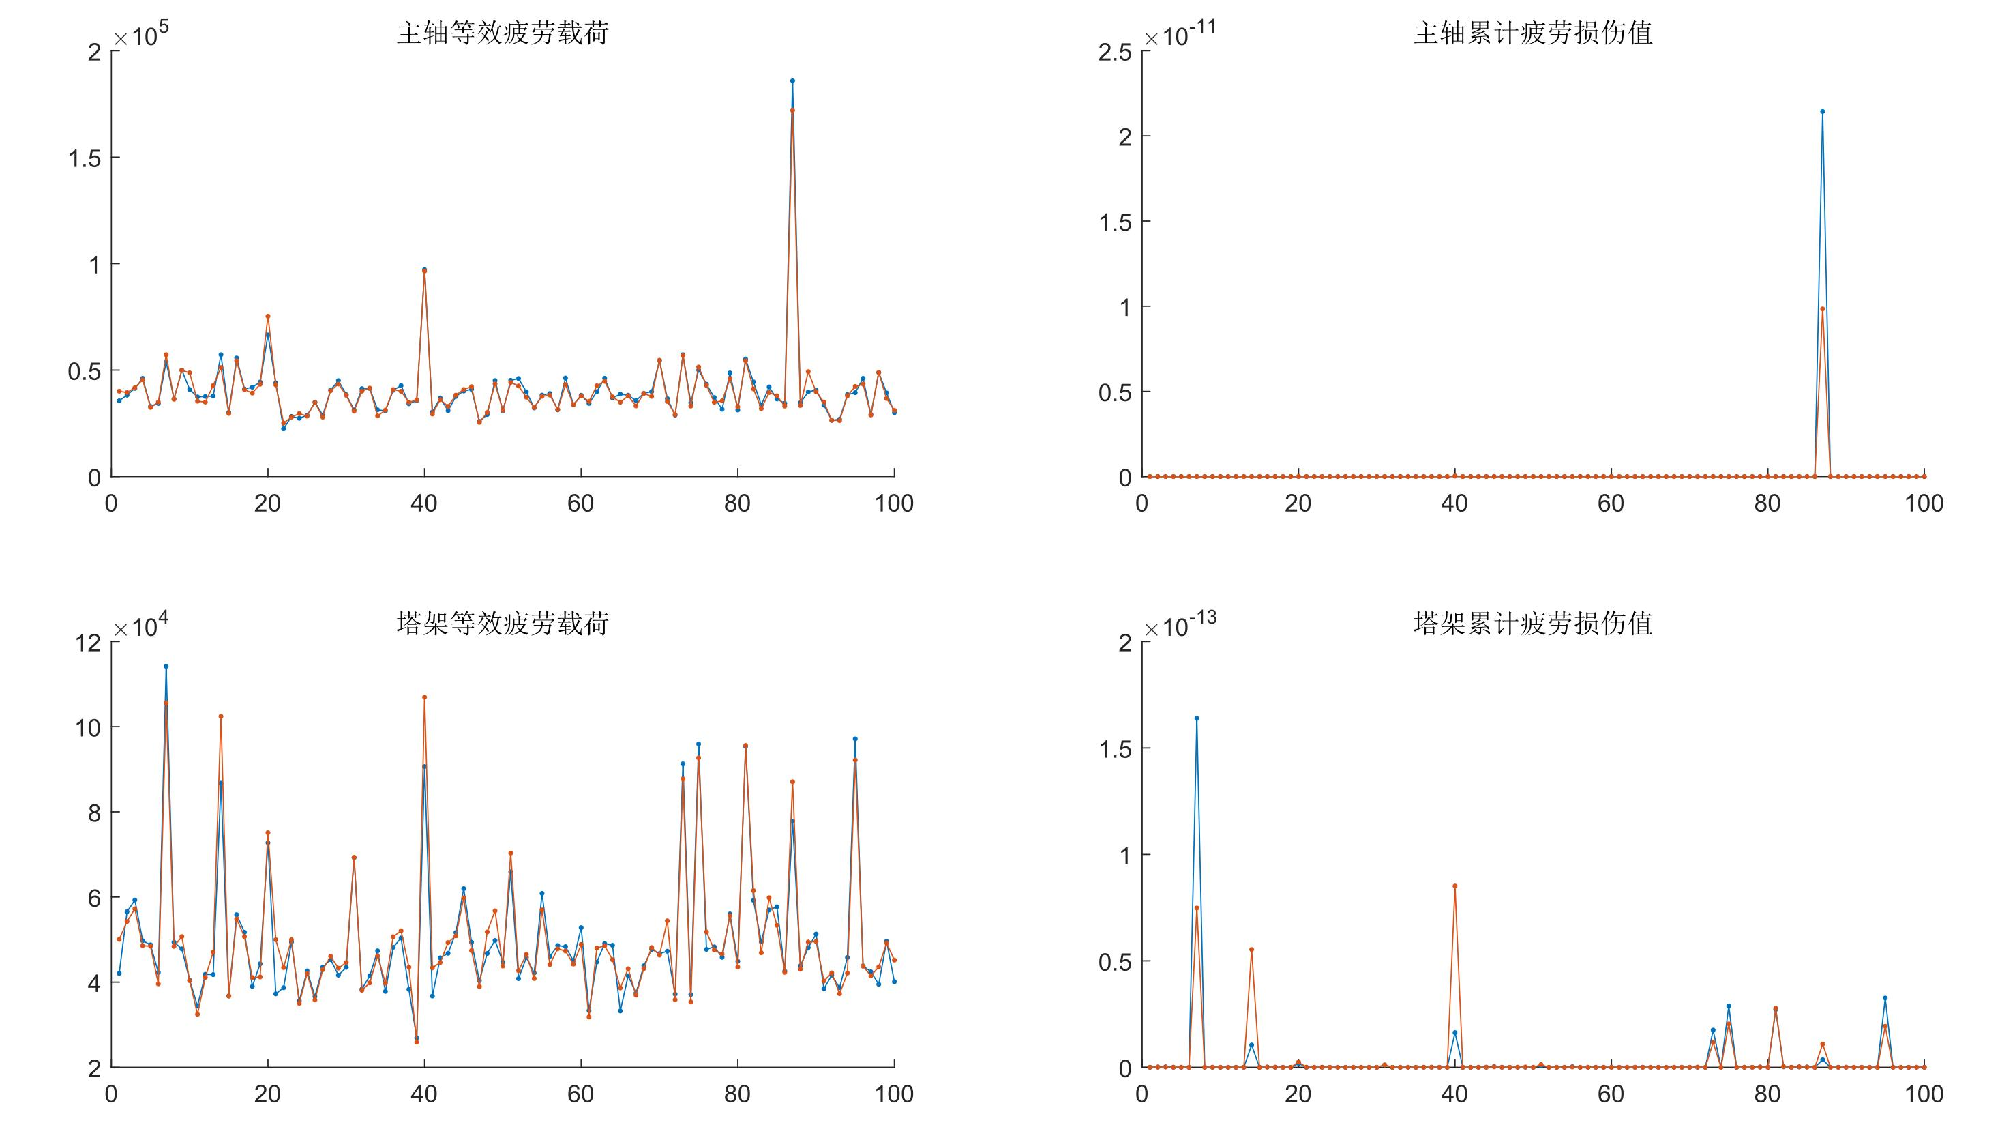
\includegraphics[width=\textwidth]{Figure_0}
	\caption{风机主轴扭矩和塔架推力等效疲劳损伤、累计疲劳损伤计算结果，其中橙色线条为参考数值，蓝色线条为模型计算数值}
	\label{fig:0}
\end{figure}
\begin{figure}[h]
	\centering
	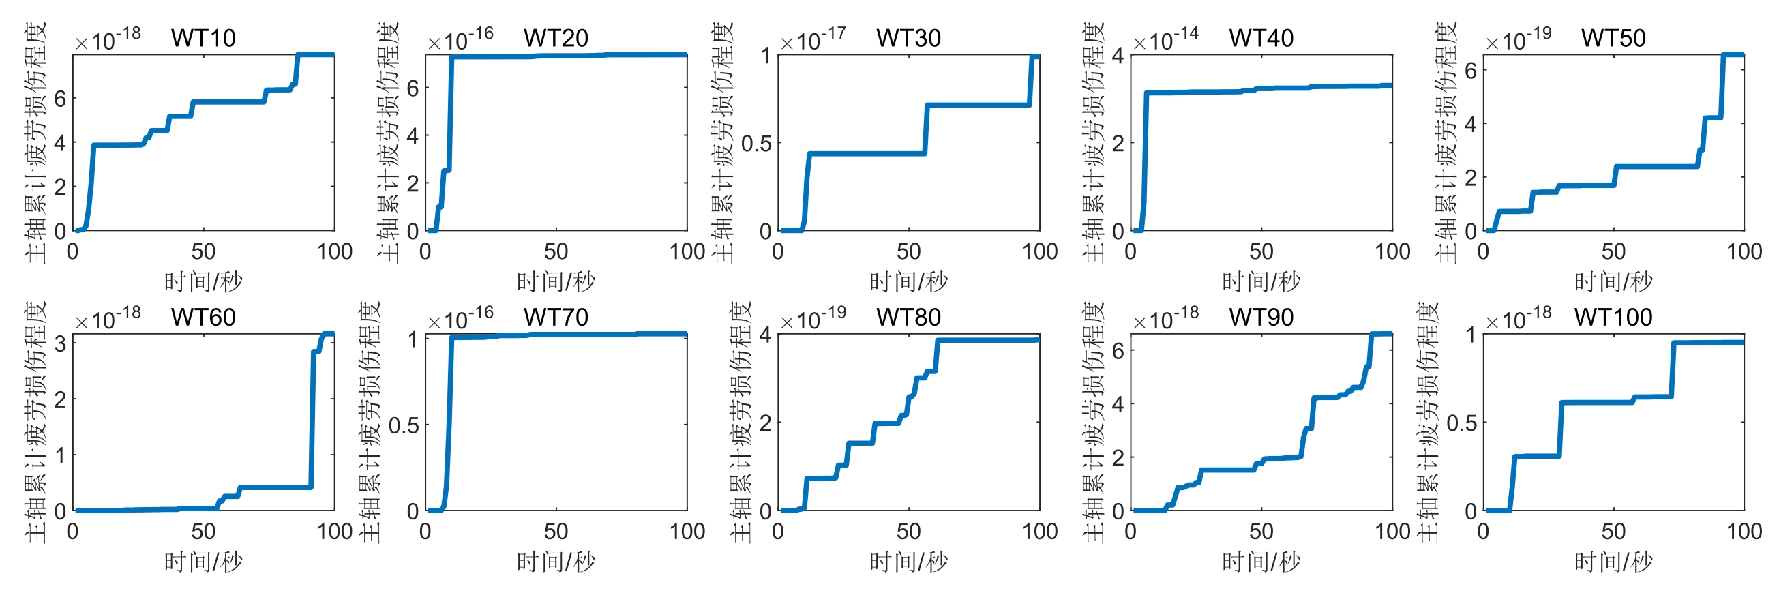
\includegraphics[width=\textwidth]{Figure_1}
	\caption{部分风机主轴扭矩累积疲劳损伤100s实时增加情况}
	\label{fig:1}
\end{figure}
\begin{figure}[h]
	\centering
	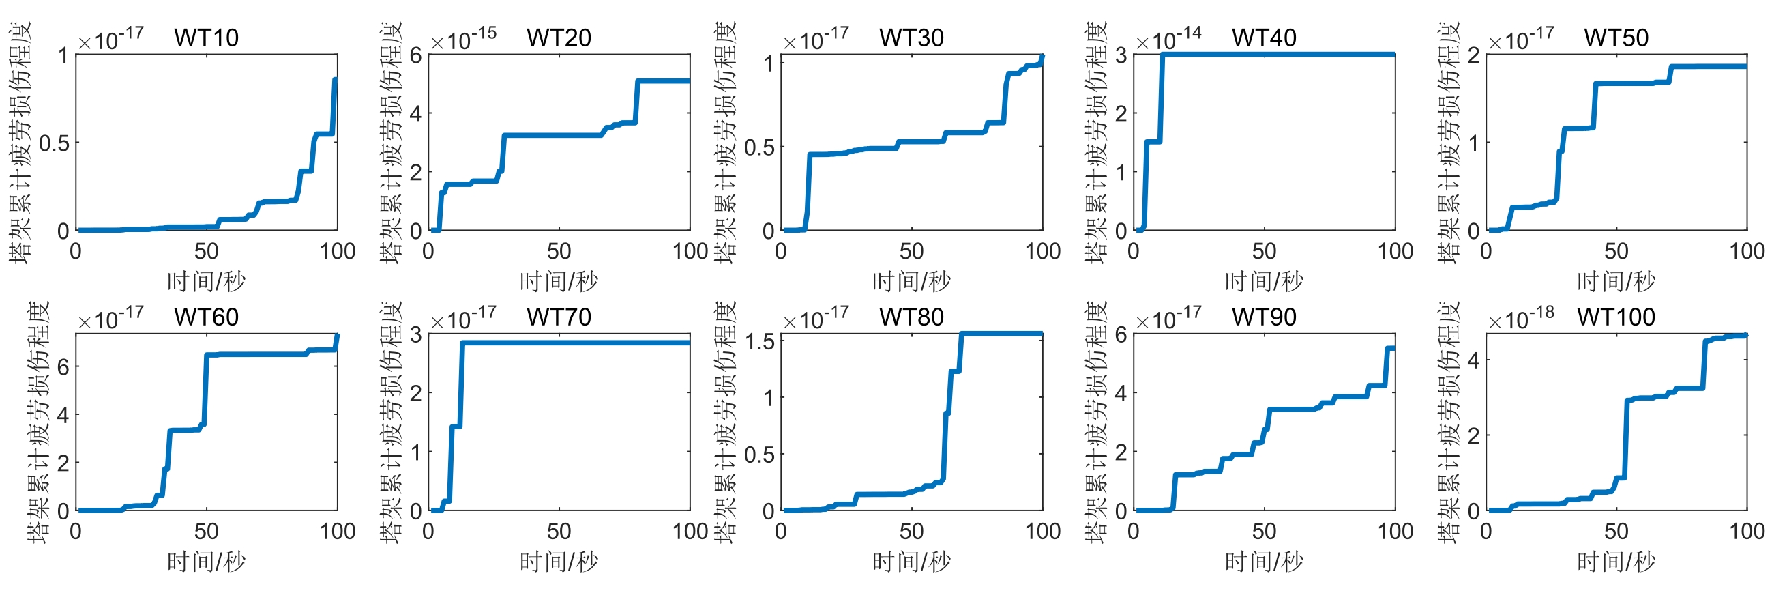
\includegraphics[width=\textwidth]{Figure_2}
	\caption{部分风机塔架推力累积疲劳损伤100s实时增加情况}
	\label{fig:2}
\end{figure}
\clearpage
\subsection{问题二：载荷计算模型}
\par \textbf{主轴扭矩}\quad 考虑指令时滞，第$i$台风机$\tau$时刻主轴扭矩
\begin{equation}
	T_s^i(\tau) = \eta\frac{P_{ref}^i(\tau-1)}{\omega_r^i},
\end{equation}
其中$\eta$为转换效率，$P_{ref}^i$和$\omega_r^i$分别为第$i$台风机的调度指令功率、低速轴转速。通过最小二乘法求解$\eta$，拟合优度$R^2=0.9691$，得到的模型为
\begin{equation}
	T_s^i(\tau) = 1.057738\frac{P_{ref}^i(\tau-1)}{\omega_r^i},
\end{equation}
\par \textbf{塔架推力}\quad 第$i$台风机塔架推力
\begin{equation}
	F_t^i = 0.5{\pi}\rho R^2C_t(\lambda_i,\beta_i)v_i^2,
\end{equation}
其中$\rho$是空气密度，$R$是风轮半径，$v_i$是风速，$C_t(\lambda_i,\beta_i)$是推力系数，
\begin{equation}
	C_t(\lambda_i,\beta_i)=c_1\left( c_2\frac{1}{\lambda _{i}^{*}}-c_5\beta _i-c_6 \right) \text{e}^{-\frac{c_7}{\lambda _{i}^{*}}}+c_8\lambda _i,
\end{equation}
其中$\lambda_i, \beta_{i}$分别是第$i$台风机叶尖速比、桨距角，满足关系
\begin{equation}
	\lambda _i=\frac{\omega _{r}^{i}R}{v_i},\quad \frac{1}{\lambda _{i}^{*}}=\frac{1}{\lambda _i+c_3\beta _i}-\frac{c_4}{\beta _{i}^{3}+1},
\end{equation}
式中$\{c_i\}_{i=1}^{8}$为待定参数。通过Levenberg-Marquardt算法拟合参数，拟合优度$R^2=0.9999$，得到的模型参数$c_3=0.0217, c_4=0.0155$, 且
\begin{equation}
	C_t(\lambda_i,\beta_i)=0.1723\left( 116.1197\frac{1}{\lambda _{i}^{*}}-1.6541\beta _i-3.2089 \right) \text{e}^{-\frac{11.4066}{\lambda _{i}^{*}}}+0.0441\lambda _i.
	\vspace{-20pt}
\end{equation}
\begin{figure}[h]
	\centering
	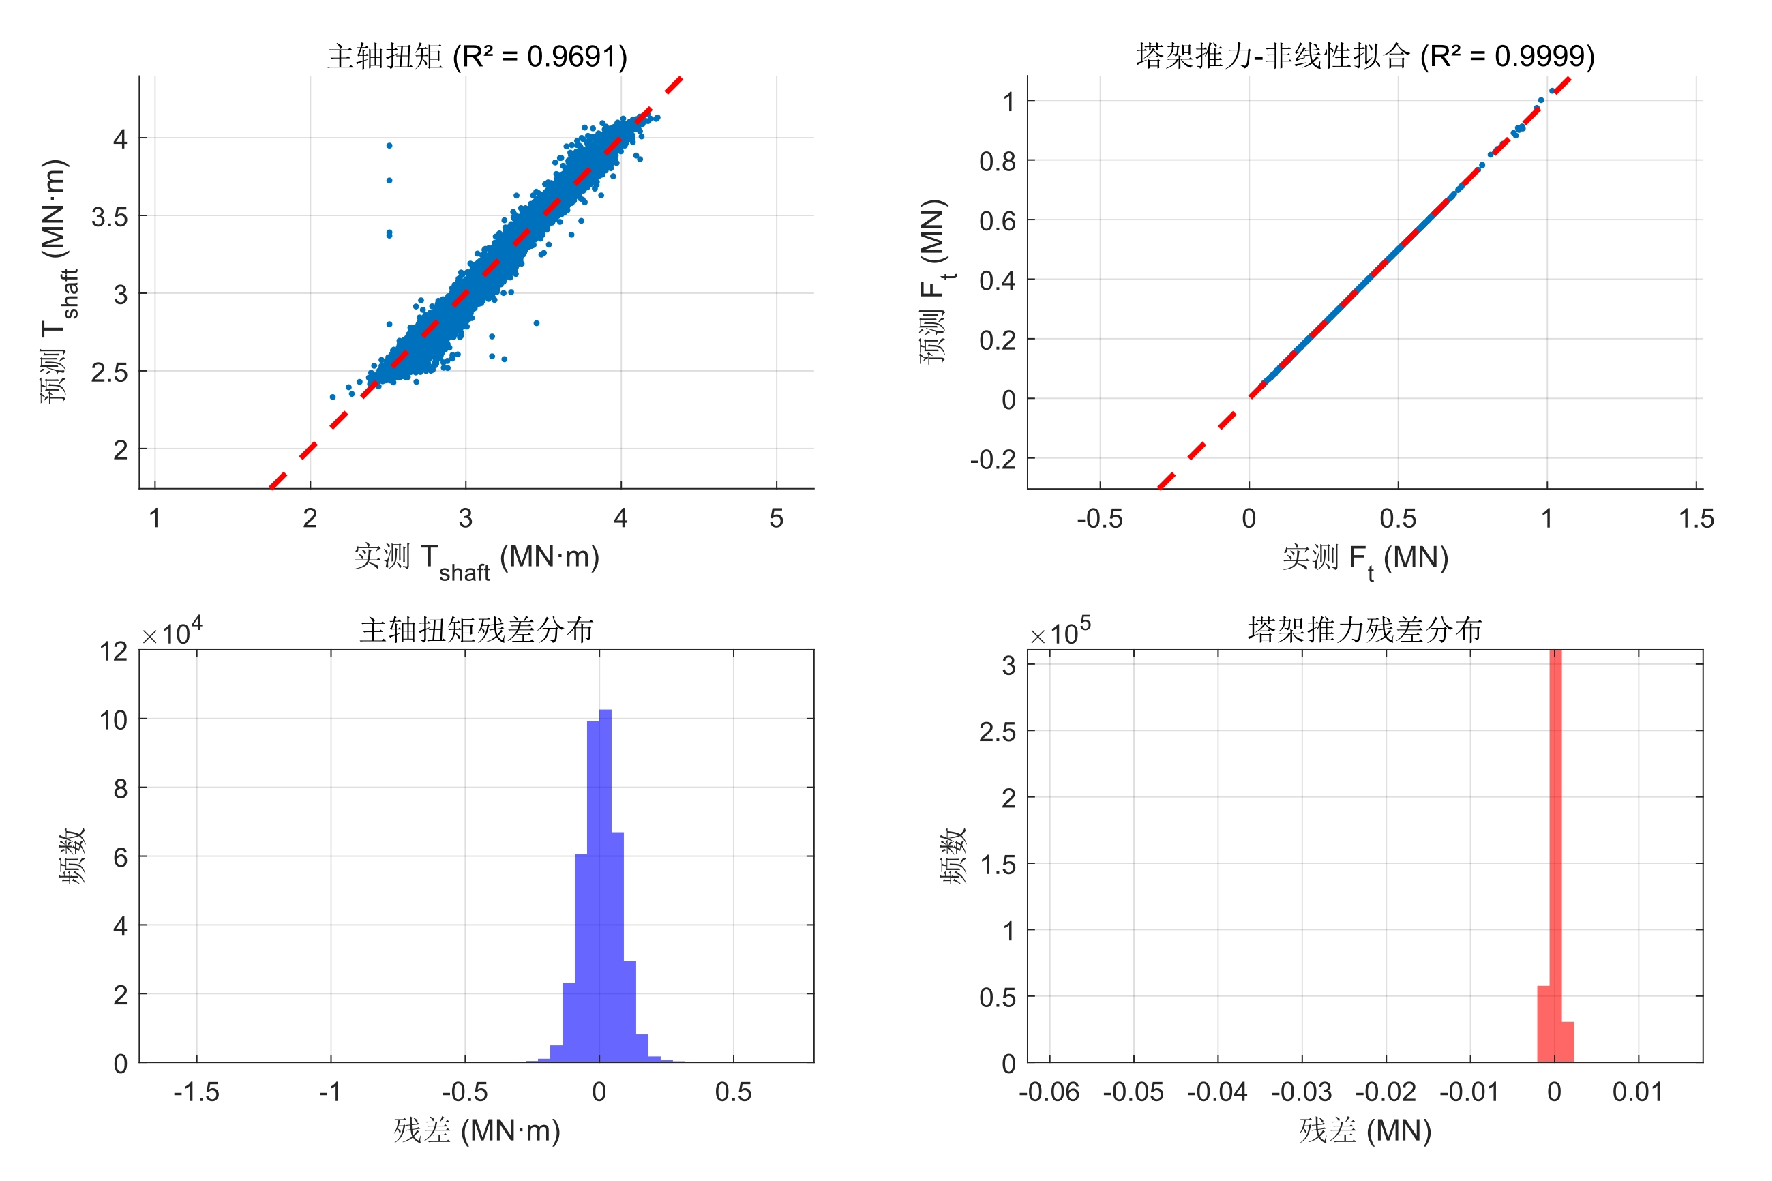
\includegraphics[width=0.8\textwidth]{Figure_3}
	\caption{风机主轴扭矩、塔架推力计算模型拟合情况}
	\label{fig:3}
	\vspace{-20pt}
\end{figure}
\clearpage
为了进一步将制定功率$P_{ref}^i$也考虑进塔架推力的模型中，修正模型为
\begin{equation}
	F_t^i(\tau) = 0.5{\pi}\rho R^2C_t(\lambda_i,\beta_i)v_i^2P_{ref}^i(\tau-1),
\end{equation}
重新拟合模型参数，拟合优度为$R^2=0.7097$，模型为
\begin{equation}
	C_t(\lambda_i,\beta_i)=0.000001\left( 115.9968\frac{1}{\lambda _{i}^{*}}-0.3942\beta _i- 5.0264\right) \text{e}^{-\frac{21.0093}{\lambda _{i}^{*}}},
\end{equation}
\begin{equation}
	\lambda _i=\frac{\omega _{r}^{i}R}{v_i},\quad \frac{1}{\lambda _{i}^{*}}=\frac{1}{\lambda _i+0.120164\beta _i}-\frac{0.026982}{\beta _{i}^{3}+1}.
\end{equation}
\subsection{问题三：优化调度模型}
\par 决策变量 
\begin{equation}
	P_{ref}^{i}(\tau), i=1,2,\cdots,100.
\end{equation}
\par 目标函数
\begin{equation}
	\min F_1 = \frac{1}{100}\sum_{i=1}^{100} D_s^i(\tau),
\end{equation}
\begin{equation}
	\min F_2 = \frac{1}{100}\sum_{i=1}^{100} D_t^i(\tau),
\end{equation}
其中
\begin{equation}
D_s^i(\tau)=\sum_{j\in\Omega^s_i(\tau)}\frac{n_s^i(j)}{N_s^i(j)},
\quad D_t^i(\tau)=\sum_{j\in\Omega^t_i(\tau)}\frac{n_t^i(j)}{N_t^i(j)},
\end{equation}
\begin{equation}
	(\hat{S}_s^i)^mN^i_s=(\hat{S}_t^i)^mN^i_t=C,
\end{equation}
\begin{equation}
	\frac{S^{i}_{s}}{\hat{S}^i_s}+\frac{\bar{S}^i_{s}}{\sigma _b}=1, \quad \frac{S^{i}_{t}}{\hat{S}^i_t}+\frac{\bar{S}^i_{t}}{\sigma _b}=1,
\end{equation}
\begin{equation}
	T_s^i(\tau) = 1.057738\frac{P_{ref}^i(\tau-1)}{\omega_r^i},
\quad 	F_t^i(\tau) = 0.5{\pi}\rho R^2C_t(\lambda_i,\beta_i)v_i^2P_{ref}^i(\tau-1),
\end{equation}
其中${S}^i_s, {S}^i_t$、$\bar{S}^i_s, \bar{S}^i_t$分别为$T_s^i, F_t^i $相应循环的幅值、均值。
\par 约束条件
\begin{align}
	\sum_{i=1}^{100} P_{ref}^i &= P_t, \\
	0 \le P_{ref}^i &\le 5, \quad \text{(MW)} \\
	|P_{ref}^i - \frac{{P}_{t}}{100}| &\le 1. \quad \text{(MW)}
\end{align}
\par 采用\textbf{多目标非支配排序遗传算法}（ Multi-Objective Non-Dominated Sorting Genetic Algorithm，简称NSGA-II）寻找Pareto最优解。
\clearpage
\begin{figure}[h]
	\centering
	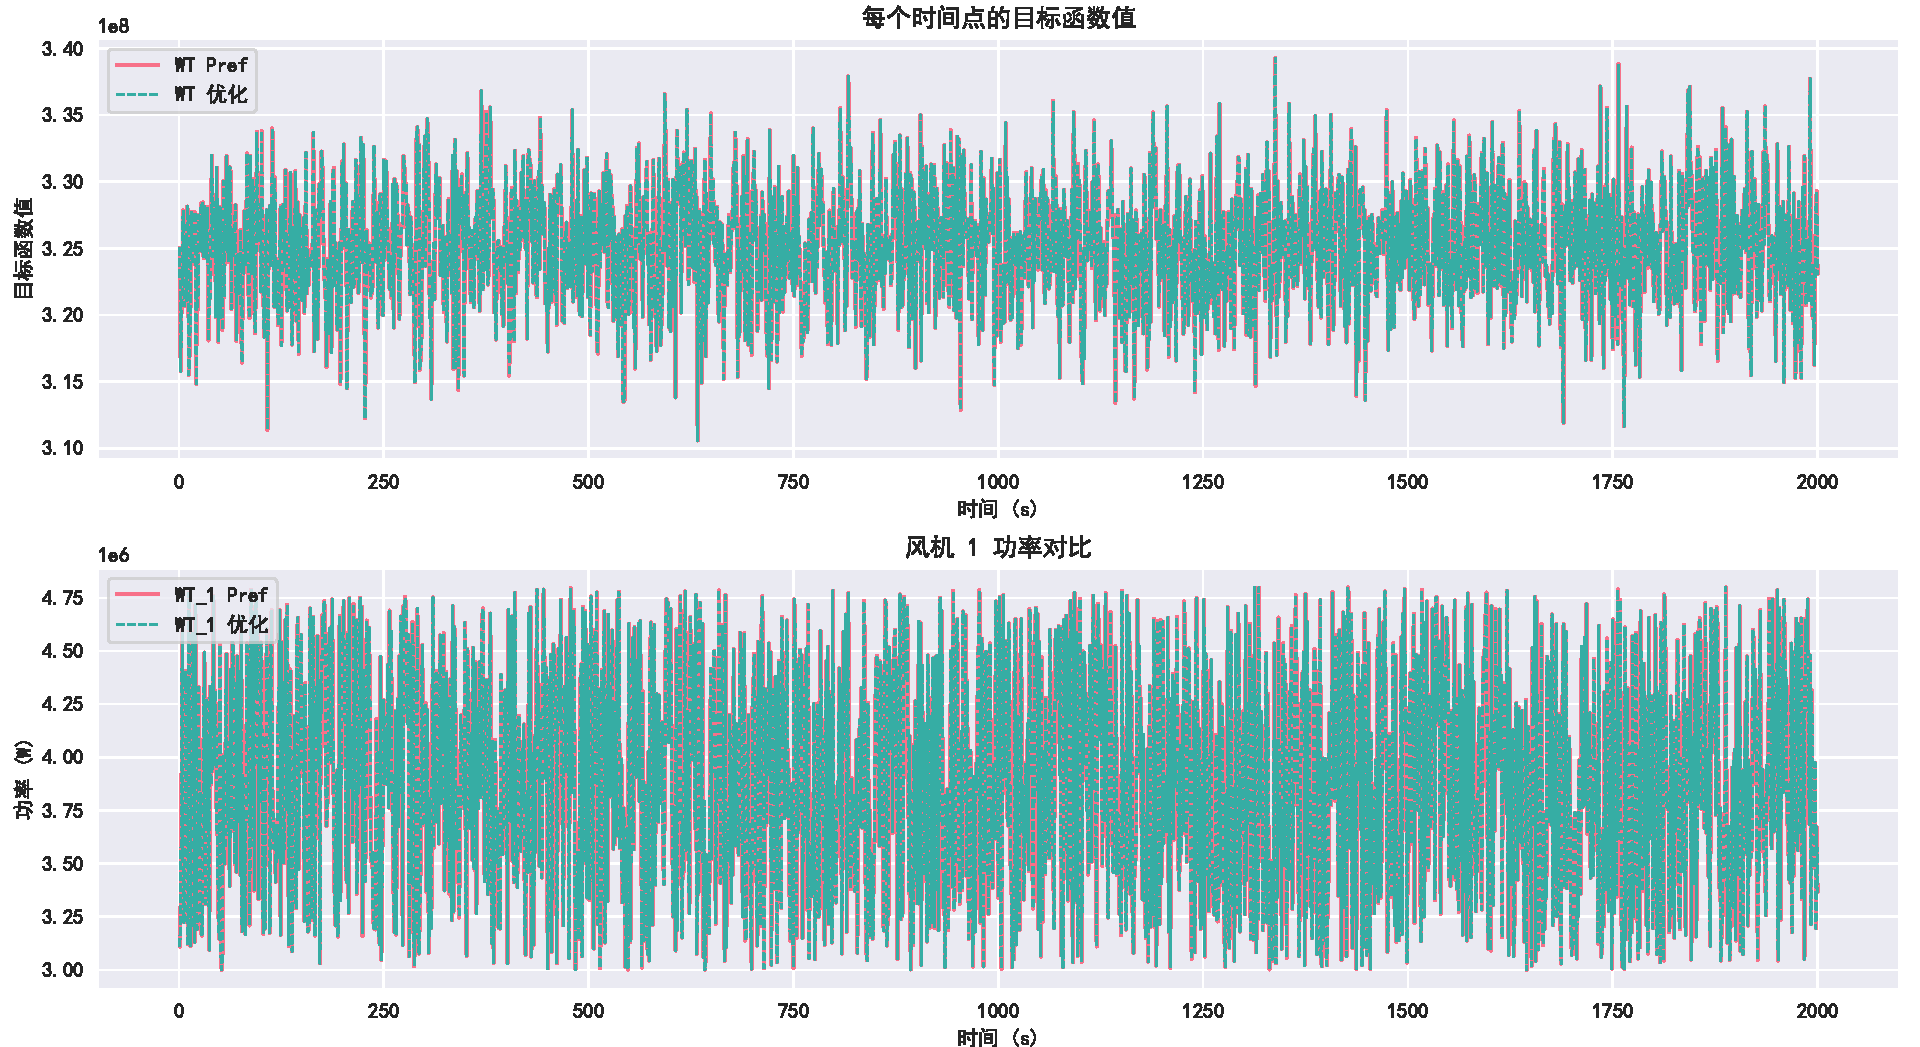
\includegraphics[width=0.95\textwidth]{Figure_4}
	\caption{NSGA-II算法优化风机功率调度前后疲劳损伤对比（t=50s）}
	\label{fig:4}
\end{figure}
\begin{figure}[h]
	\centering
	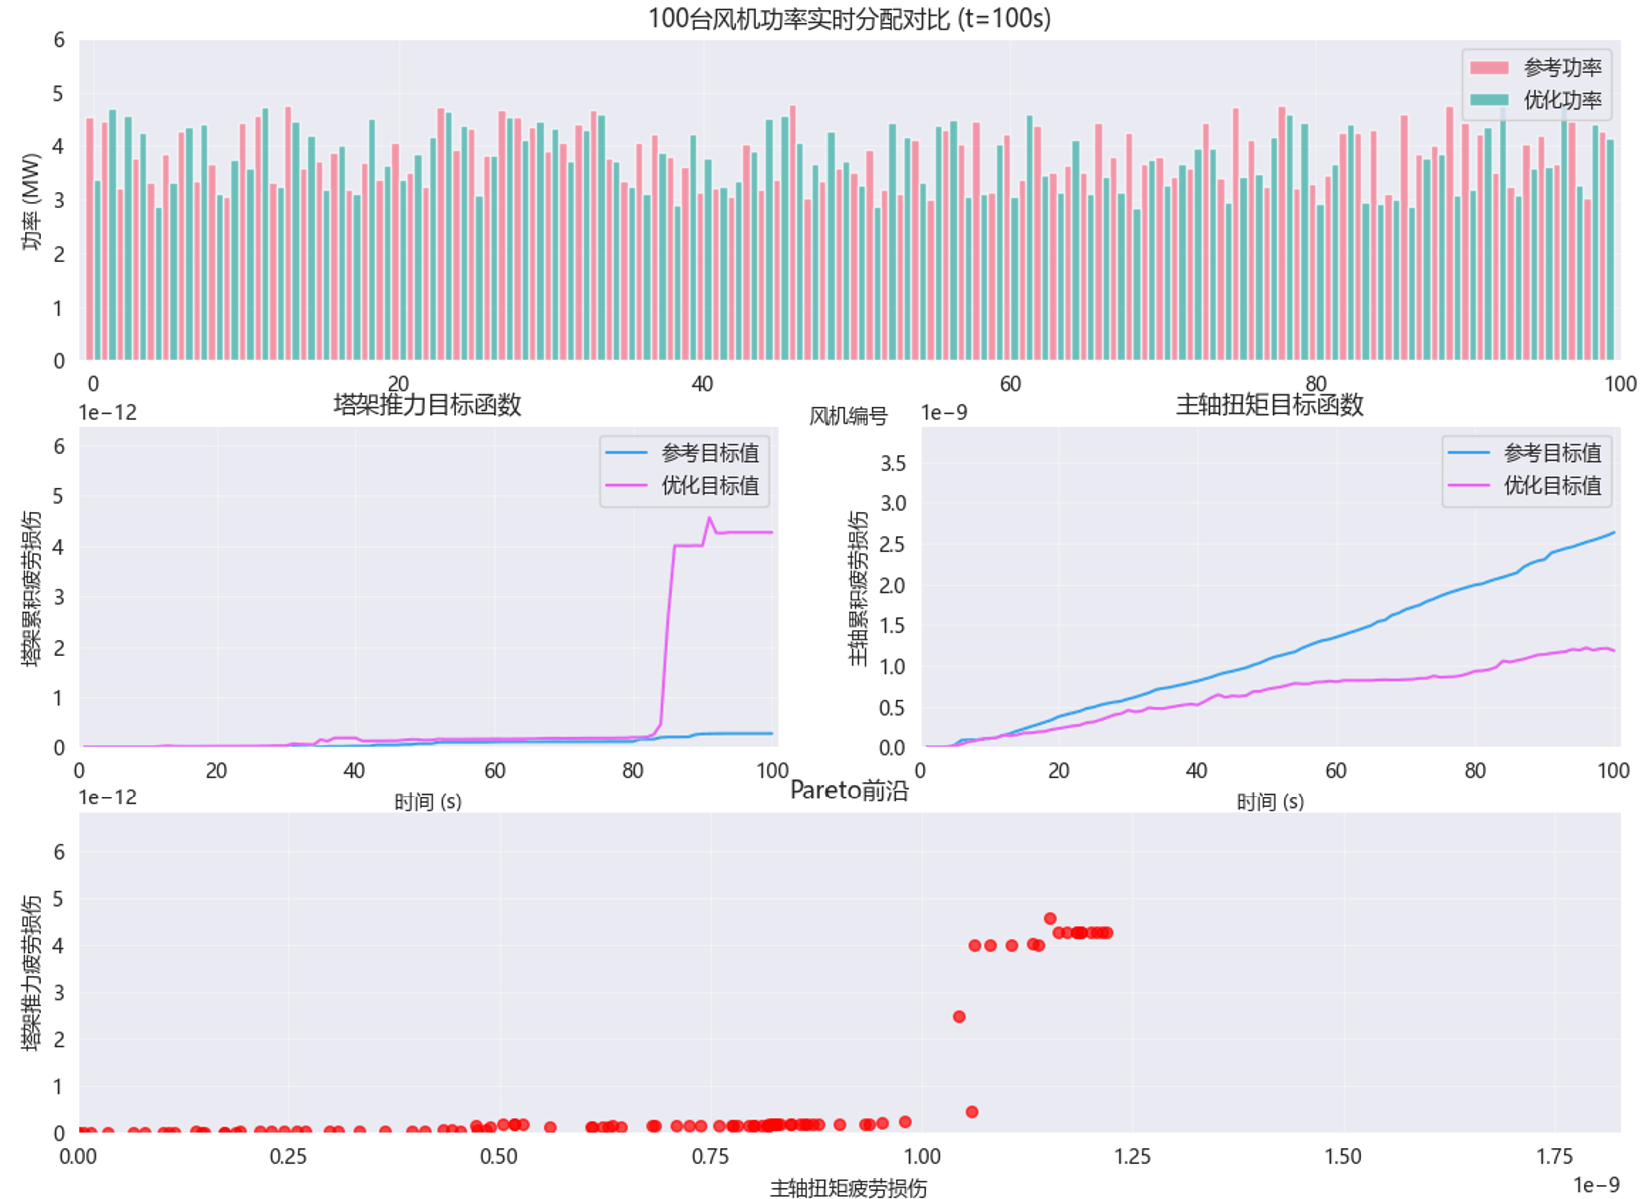
\includegraphics[width=0.95\textwidth]{Figure_5}
	\caption{NSGA-II算法优化风机功率调度前后疲劳损伤对比（t=100s）}
	\vspace{-20pt}
	\label{fig:5}
\end{figure}
\newpage
\noindent 注： 采用序列最小二乘规划（SLSQP）方法单独求解各目标，结果如图所示。
\begin{figure}[h]
	\centering
	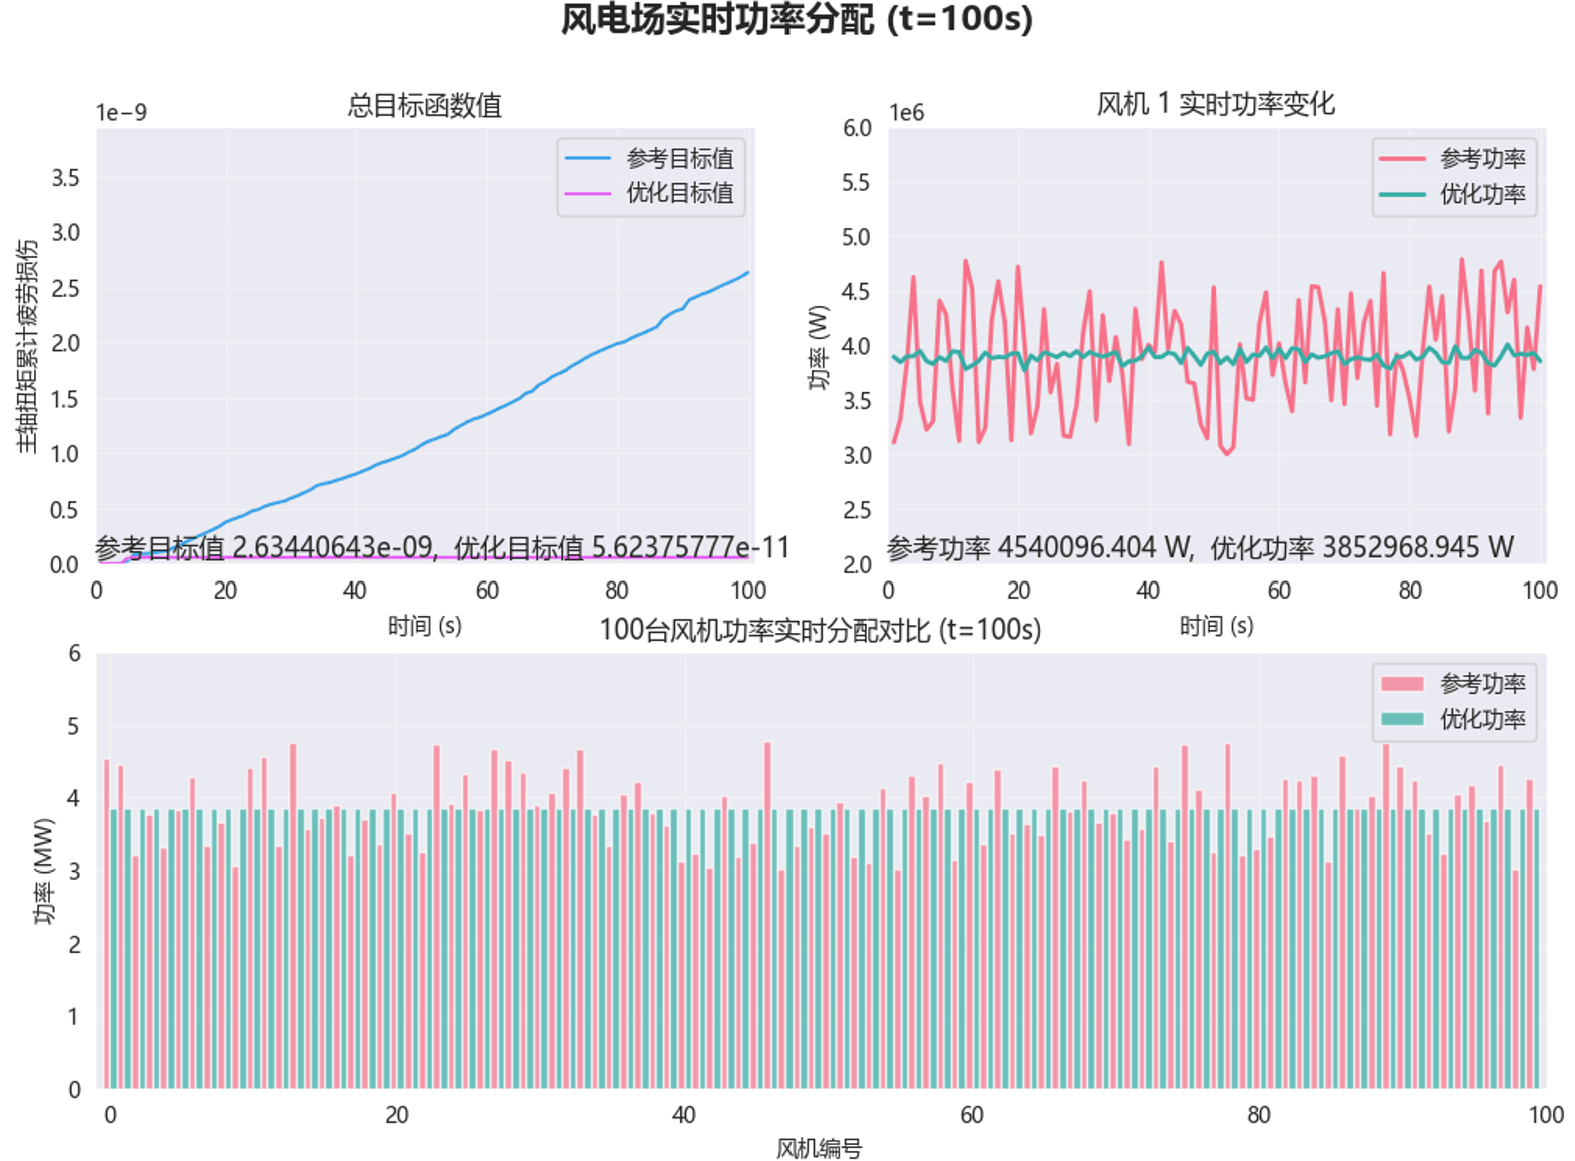
\includegraphics[width=0.9\textwidth]{Figure_6}
	\caption{风机功率调度优化前后塔架推力疲劳损伤对比}
	\label{fig:6}
\end{figure}
\begin{figure}[h]
	\centering
	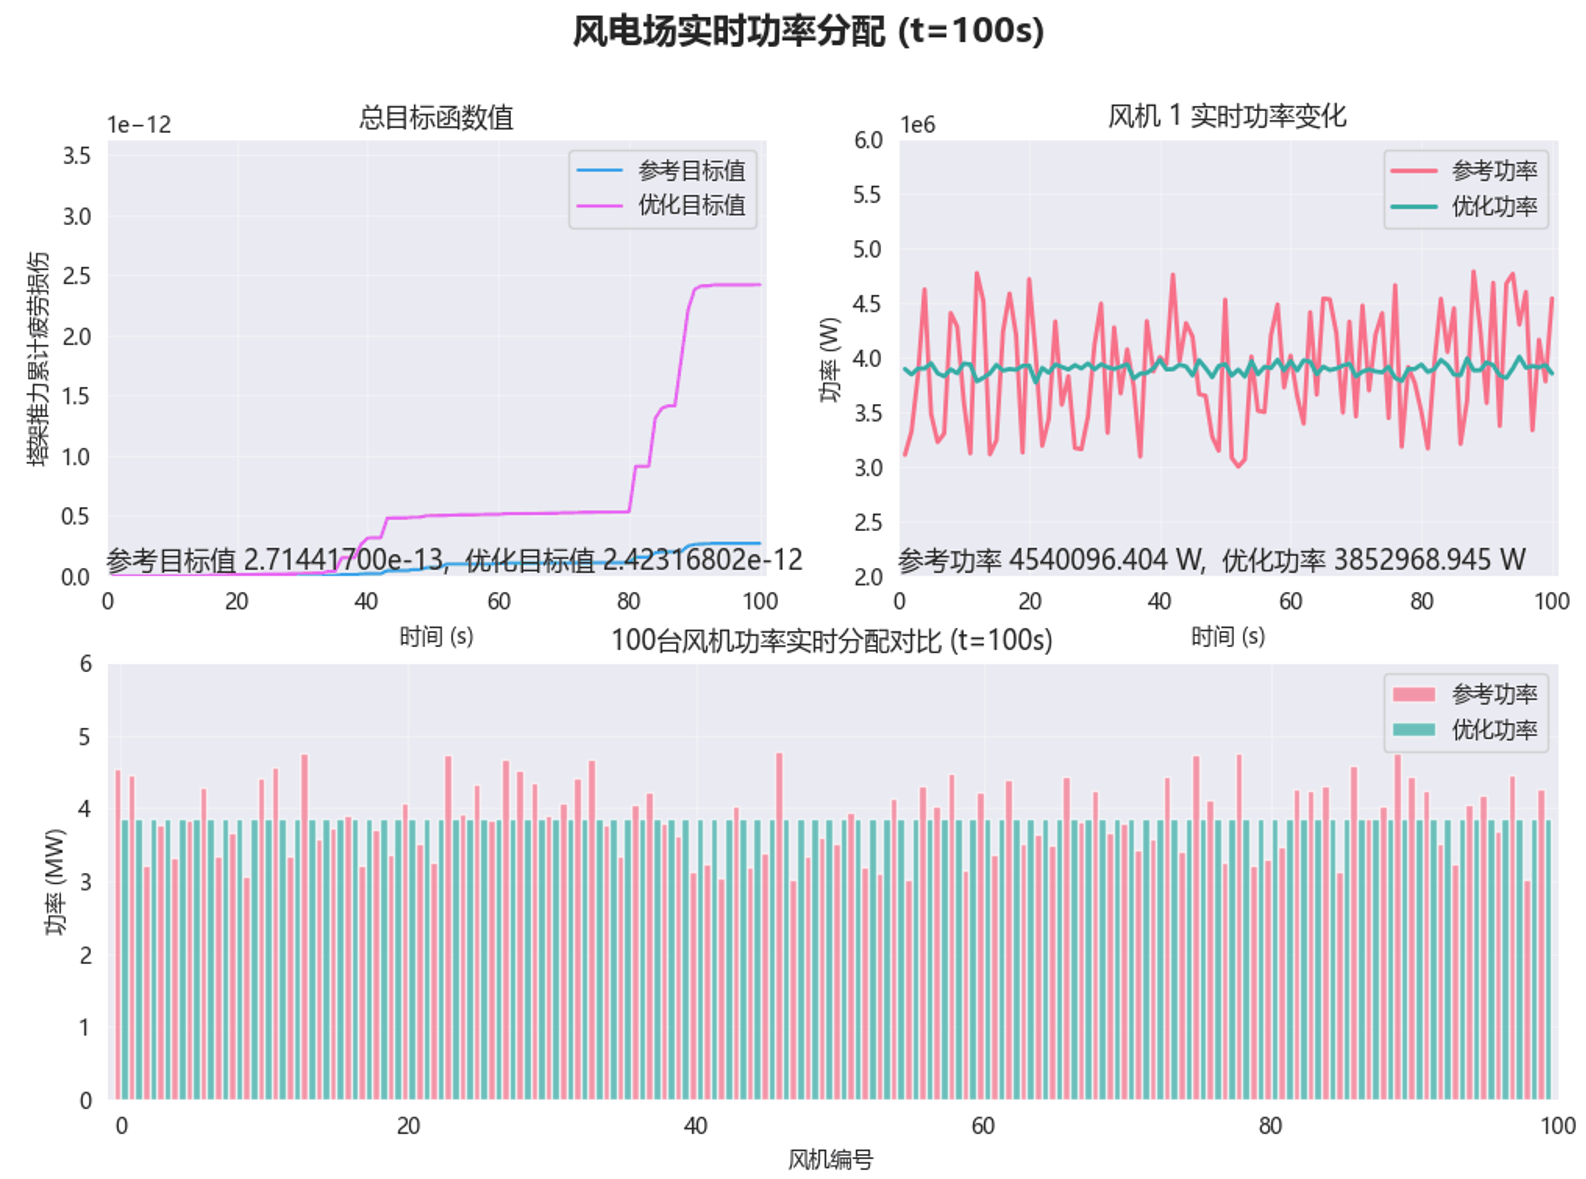
\includegraphics[width=0.9\textwidth]{Figure_7}
	\caption{风机功率调度优化前后主轴扭矩疲劳损伤对比}
	\label{fig:7}
\end{figure}
\newpage
\subsection{问题四：鲁棒优化模型}
卡尔曼滤波假设系统状态随时间线性演化，且观测值带有高斯白噪声，通过最小化估计误差的协方差，在“物理模型预测”和“含噪传感器测量”之间找到最优平衡，给出状态的最优估计。
\par \textbf{状态预测（先验估计） }
根据上一时刻的最优估计，预测当前时刻的状态：
\[
\hat{x}_{k|k-1} = A \hat{x}_{k-1|k-1} + B u_{k-1}
\]
同时预测误差协方差：
\[
P_{k|k-1} = A P_{k-1|k-1} A^T + Q
\]
其中\(A\)是状态转移矩阵，\(B\)是控制输入，\(u\)是外部输入，  
\(Q\)是过程噪声协方差。
\par\textbf{ 测量更新（后验校正） }
利用当前观测 \(z_k\) 修正预测值：
\begin{itemize}
	\item 计算卡尔曼增益：
	\[
	K_k = P_{k|k-1} H^T (H P_{k|k-1} H^T + R)^{-1}
	\]
	\item 状态更新：
	\[
	\hat{x}_{k|k} = \hat{x}_{k|k-1} + K_k (z_k - H \hat{x}_{k|k-1})
	\]
	\item 误差协方差更新：
	\[
	P_{k|k} = (I - K_k H) P_{k|k-1}
	\]
	其中\(H\)是观测矩阵，\(R\)是测量噪声协方差。
\end{itemize}
\begin{figure}[h]
	\centering
	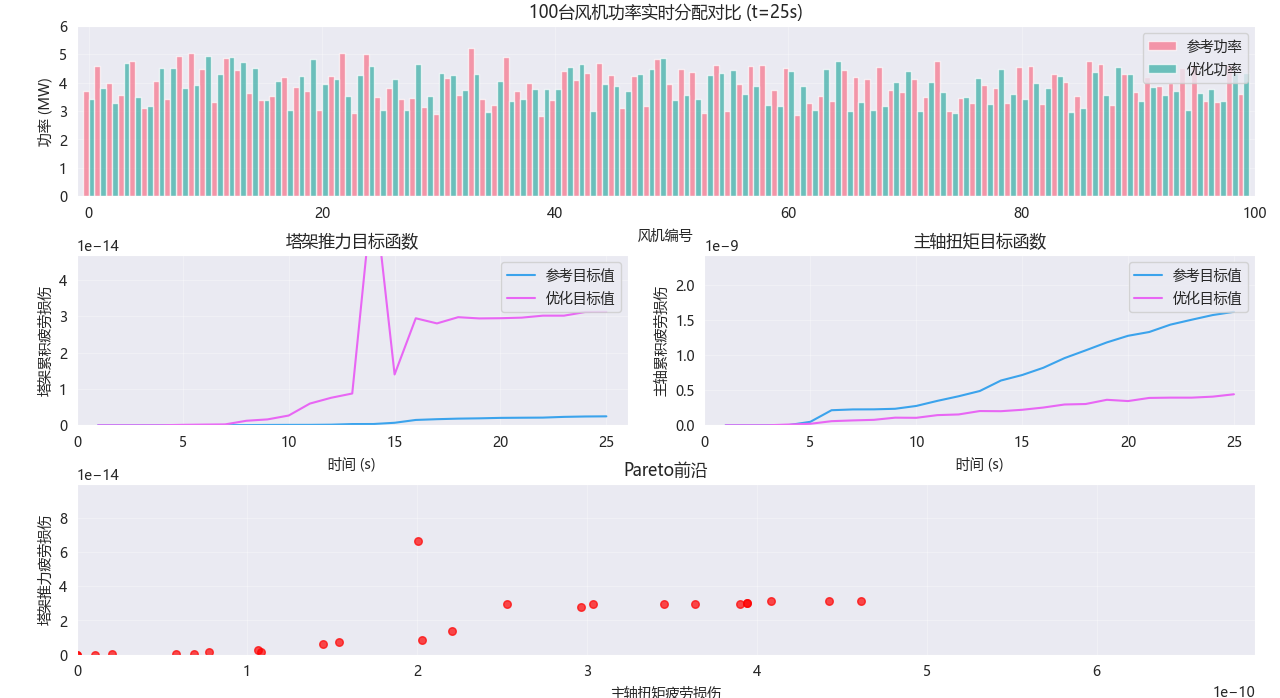
\includegraphics[width=0.95\textwidth]{Figure_8}
	\caption{基于卡尔曼滤波与时滞补偿的优化调度前后疲劳损伤对比（t=25s）}
	\label{fig:8}
\end{figure}

\section{参考文献}
\begin{thebibliography}{99}
	\bibitem{1} Musallam M, Johnson C M. An efficient implementation of the rainflow counting algorithm for life consumption estimation. \textit{IEEE Trans. Rel.}, 2012, 61(4): 978-986.
	\bibitem{2} 董乐义, 罗俊. 雨流计数法及其在程序中的具体实现[J]. 计算机技术与应用, 2004, 24(3): 38-40.
	\bibitem{3} 王宏伟. 雨流计数法及其在疲劳寿命估算中的应用[J]. 矿山机械, 2006, 34(3): 95-97.
	\bibitem{4} 姚琦,胡阳,柳玉等.考虑载荷抑制的风电场分布式自动发电控制[J]. 电工技术学报, 2022, 37(3): 697-706.
\end{thebibliography}
\end{document} 
